\documentclass[12pt]{article}

\usepackage{graphicx}% Include figure files
\usepackage{dcolumn}% Align table columns on decimal point

% Use Arial font %
\usepackage{helvet}
\renewcommand{\familydefault}{\sfdefault} 

% Default margins and paper properties %
\usepackage[a4, portrait, margin=0.6in]{geometry}

\begin{document}
	\title{Hypothesis plots summary} % Force line breaks with \\
	\author{1666957, Gustavo Espinal Lugo}
	\date{\today} % It is always \today, today, %  but any date may be explicitly specified

	\maketitle
	%\tableofcontents
	
	\section*{Plots and corresponding metadata}
	mean expected W mass: 80.379 $[GeV/c^{2}]$,\\
mean hypothesis masses: [78.  78.5 79.  79.5 80.  80.5 81.  81.5 82. ] $[GeV/c^{2}]$,\\
mass width: 2.07 $[GeV/c^{2}]$,\\
chi\_square value of hypothesis fit: 1.66036052363519\\
	Absolute path to figure: /home/physics/phuxdp/Desktop/PX402 Physics Project/WBosonProject/T2W5/plots/muPT\_80.379\_2.07\_between\_78\_and\_82\_summary.png\\
	Next lines are the data of the shown histograms (if needed): \\
	All quantities: 	80.379, [78.  78.5 79.  79.5 80.  80.5 81.  81.5 82. ], 2070, 1.66036052363519\\
	X\_energ\_vls = [0.6, 1.7999999999999998, 3.0, 4.199999999999999, 5.4, 6.6, 7.8, 9.0, 10.2, 11.399999999999999, 12.6, 13.799999999999999, 15.0, 16.2, 17.4, 18.6, 19.799999999999997, 21.0, 22.2, 23.4, 24.6, 25.799999999999997, 27.0, 28.199999999999996, 29.4, 30.6, 31.799999999999997, 33.0, 34.2, 35.4, 36.599999999999994, 37.8, 39.0, 40.2, 41.4, 42.599999999999994, 43.8, 45.0, 46.2, 47.4, 48.599999999999994, 49.8, 51.0, 52.2, 53.4, 54.599999999999994, 55.8, 57.0, 58.199999999999996, 59.4, 60.599999999999994, 61.8, 63.0, 64.19999999999999, 65.4, 66.6, 67.8, 69.0, 70.19999999999999, 71.4, 72.6, 73.8, 75.0, 76.19999999999999, 77.4, 78.6, 79.8, 81.0, 82.19999999999999, 83.4, 84.6, 85.8, 87.0, 88.19999999999999, 89.4, 90.6, 91.8, 93.0, 94.19999999999999, 95.4, 96.6, 97.8, 99.0, 100.19999999999999, 101.4, 102.6, 103.8, 105.0, 106.19999999999999, 107.4, 108.6, 109.8, 111.0, 112.19999999999999, 113.4, 114.6, 115.79999999999998, 117.0, 118.19999999999999, 119.4]\\
	Y\_data\_bin\_cnts = [0.0, 0.0, 0.0, 0.0, 0.0, 0.0, 0.0, 0.0, 0.0, 0.0, 0.0, 0.0, 0.0, 0.0, 0.0, 0.0, 0.0, 0.0, 9.1775541305542, 526.7265014648438, 659.4212646484375, 670.2781982421875, 721.2316284179688, 710.2410278320312, 697.9017944335938, 699.541015625, 708.6096801757812, 721.0978393554688, 741.461181640625, 719.168212890625, 647.0701293945312, 648.0154418945312, 574.1846313476562, 424.4632568359375, 355.417724609375, 264.8435974121094, 194.87930297851562, 174.15440368652344, 123.42887878417969, 113.54820251464844, 99.77728271484375, 73.01136779785156, 53.351383209228516, 71.44650268554688, 49.2791862487793, 51.009803771972656, 28.026636123657227, 27.119930267333984, 24.276813507080078, 29.108312606811523, 21.137189865112305, 23.120773315429688, 26.21957778930664, 26.864591598510742, 14.509918212890625, 19.5084228515625, 10.61483097076416, 9.702730178833008, 6.131746768951416, 7.1539130210876465, 9.36469554901123, 9.290584564208984, 11.457411766052246, 8.552010536193848, 5.086819648742676, 10.632268905639648, 5.185015678405762, 3.310250997543335, 6.952884674072266, 4.1780924797058105, 2.1605124473571777, 3.240140676498413, 4.271215438842773, 4.133248805999756, 3.2526426315307617, 2.1902503967285156, 3.0861306190490723, 1.0014219284057617, 1.0765730142593384, 3.1867599487304688, 0.0, 4.118042945861816, 1.0384154319763184, 1.0001643896102905, 1.0820047855377197, 1.0122246742248535, 2.182573080062866, 0.0, 0.0, 1.0704058408737183, 0.0, 1.0167871713638306, 1.0493755340576172, 0.0, 0.0, 0.0, 0.0, 1.038958191871643, 2.357518196105957, 0.0]\\
	Y\_model\_bin\_cnts = [0.0, 0.0, 0.0, 0.0, 0.0, 0.0, 0.0, 0.0, 0.0, 0.0, 0.0, 0.0, 0.0, 0.0, 0.0, 0.0, 0.0, 0.0, 13.546685218811035, 505.22882080078125, 613.6394653320312, 648.259765625, 656.5174560546875, 659.80126953125, 661.6873779296875, 686.786865234375, 741.6969604492188, 756.8272094726562, 691.4217529296875, 665.1148071289062, 634.1113891601562, 594.419921875, 512.5458374023438, 441.5511779785156, 332.1221618652344, 252.7998046875, 211.77223205566406, 164.1638641357422, 156.94244384765625, 105.50464630126953, 100.84651184082031, 67.80235290527344, 67.78861999511719, 57.344749450683594, 37.711708068847656, 45.119380950927734, 45.33501052856445, 27.59003257751465, 37.922550201416016, 26.203685760498047, 25.349470138549805, 18.950607299804688, 21.776824951171875, 20.378137588500977, 18.362878799438477, 15.919631004333496, 13.274507522583008, 9.177451133728027, 6.414327621459961, 5.064396381378174, 5.942914009094238, 11.034195899963379, 7.036373138427734, 4.064119338989258, 10.099827766418457, 6.298214912414551, 6.981692790985107, 7.205685615539551, 5.0517096519470215, 2.9985013008117676, 5.903761863708496, 3.108635663986206, 2.9623405933380127, 0.0, 2.991978406906128, 2.901911497116089, 0.9625916481018066, 6.985177040100098, 2.8949034214019775, 1.9509077072143555, 2.005769729614258, 0.9759769439697266, 0.9609125256538391, 1.0275695323944092, 1.1519839763641357, 1.9388151168823242, 1.019948124885559, 0.0, 1.9340468645095825, 0.0, 0.9719834327697754, 0.0, 1.95217764377594, 1.9436113834381104, 0.0, 0.9646351933479309, 2.9358010292053223, 0.0, 0.9703799486160278, 0.0]\\

    Found optimal massses ($\chi^2$ roots): [81.111902] $[GeV/c^{2}]$
    Uncertainty [GeV/c^2]: 0.0

	\begin{figure}[tb]
		\centering
		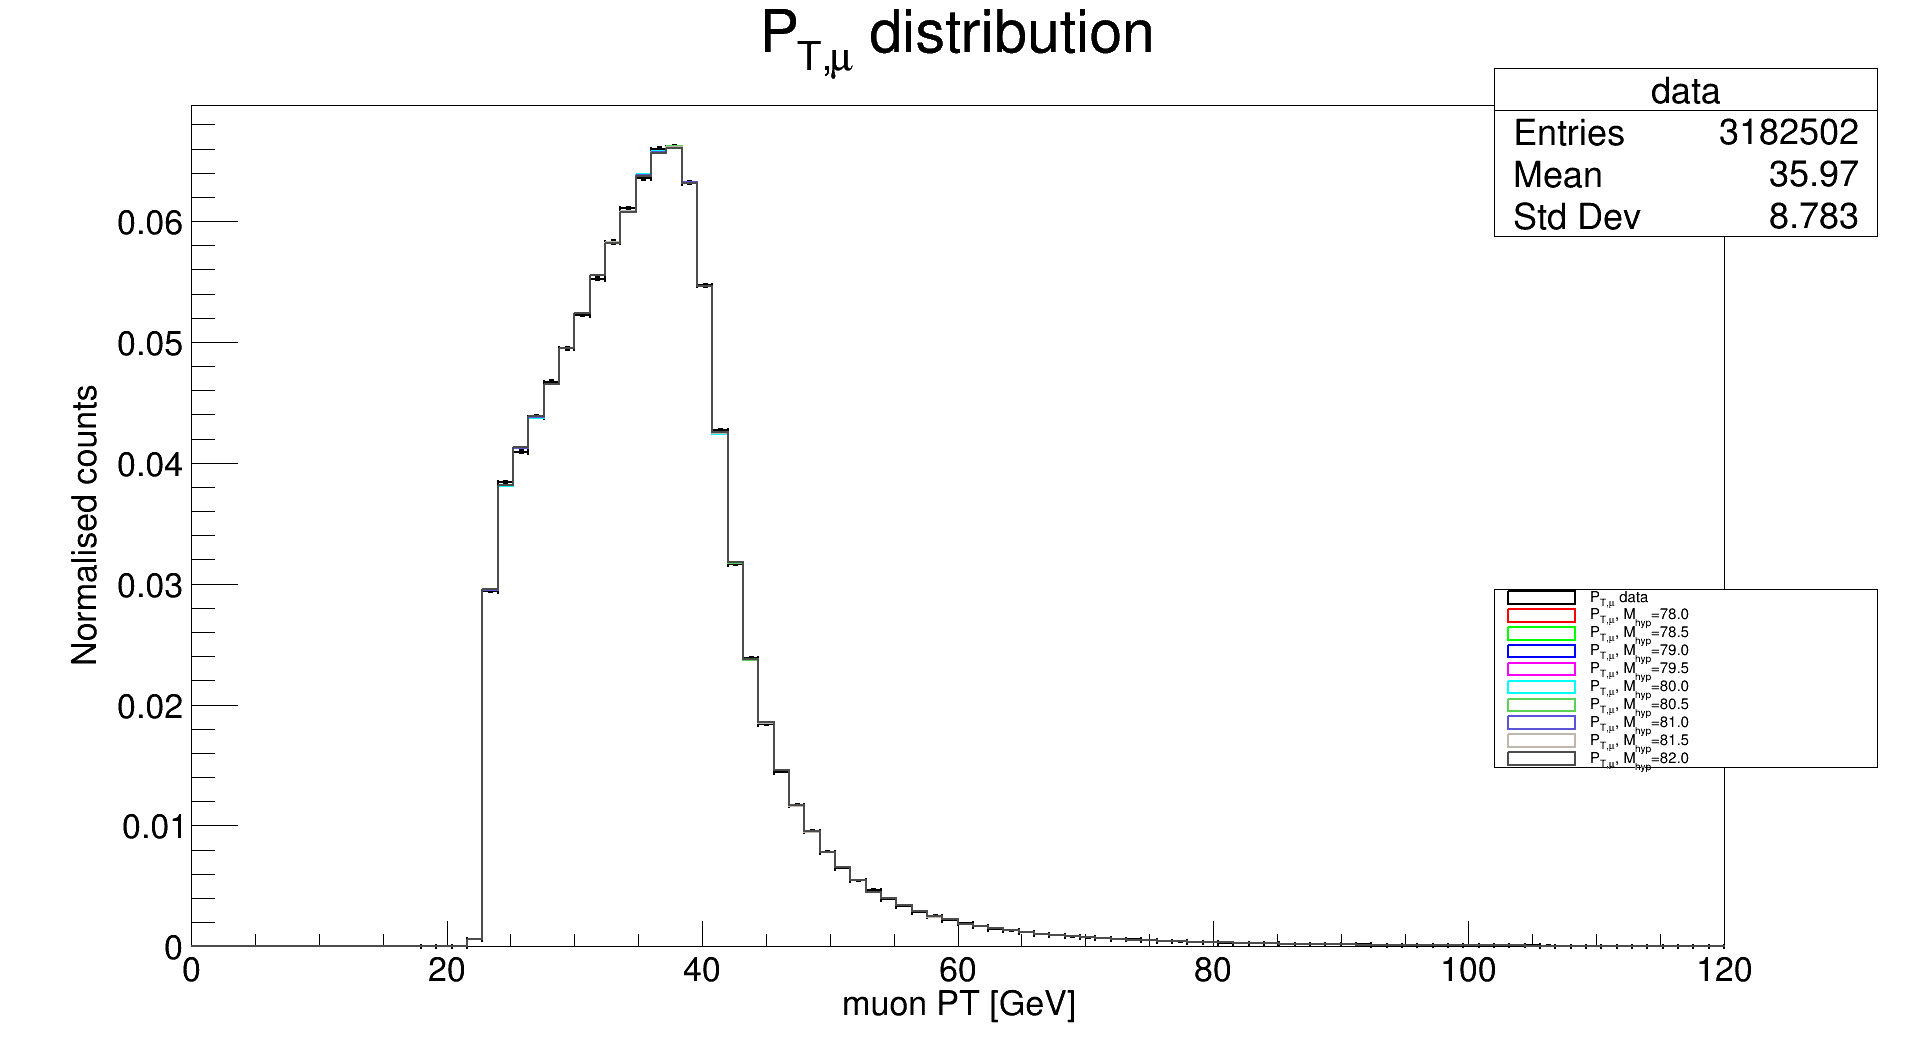
\includegraphics[width=\columnwidth]{/home/physics/phuxdp/Desktop/PX402 Physics Project/WBosonProject/T2W5/plots/muPT_80.379_2.07_between_78_and_82_summary.png}
		\caption{\small Hypothesis masses mean expected W mass: 80.379 $[GeV/c^{2}]$,\\
mean hypothesis masses: [78.  78.5 79.  79.5 80.  80.5 81.  81.5 82. ] $[GeV/c^{2}]$,\\
mass width: 2.07 $[GeV/c^{2}]$,\\
chi_square value of hypothesis fit: 1.66036052363519. }
		\label{fig: fig_0}
	\end{figure}

       \begin{figure}[tb]
		\centering
		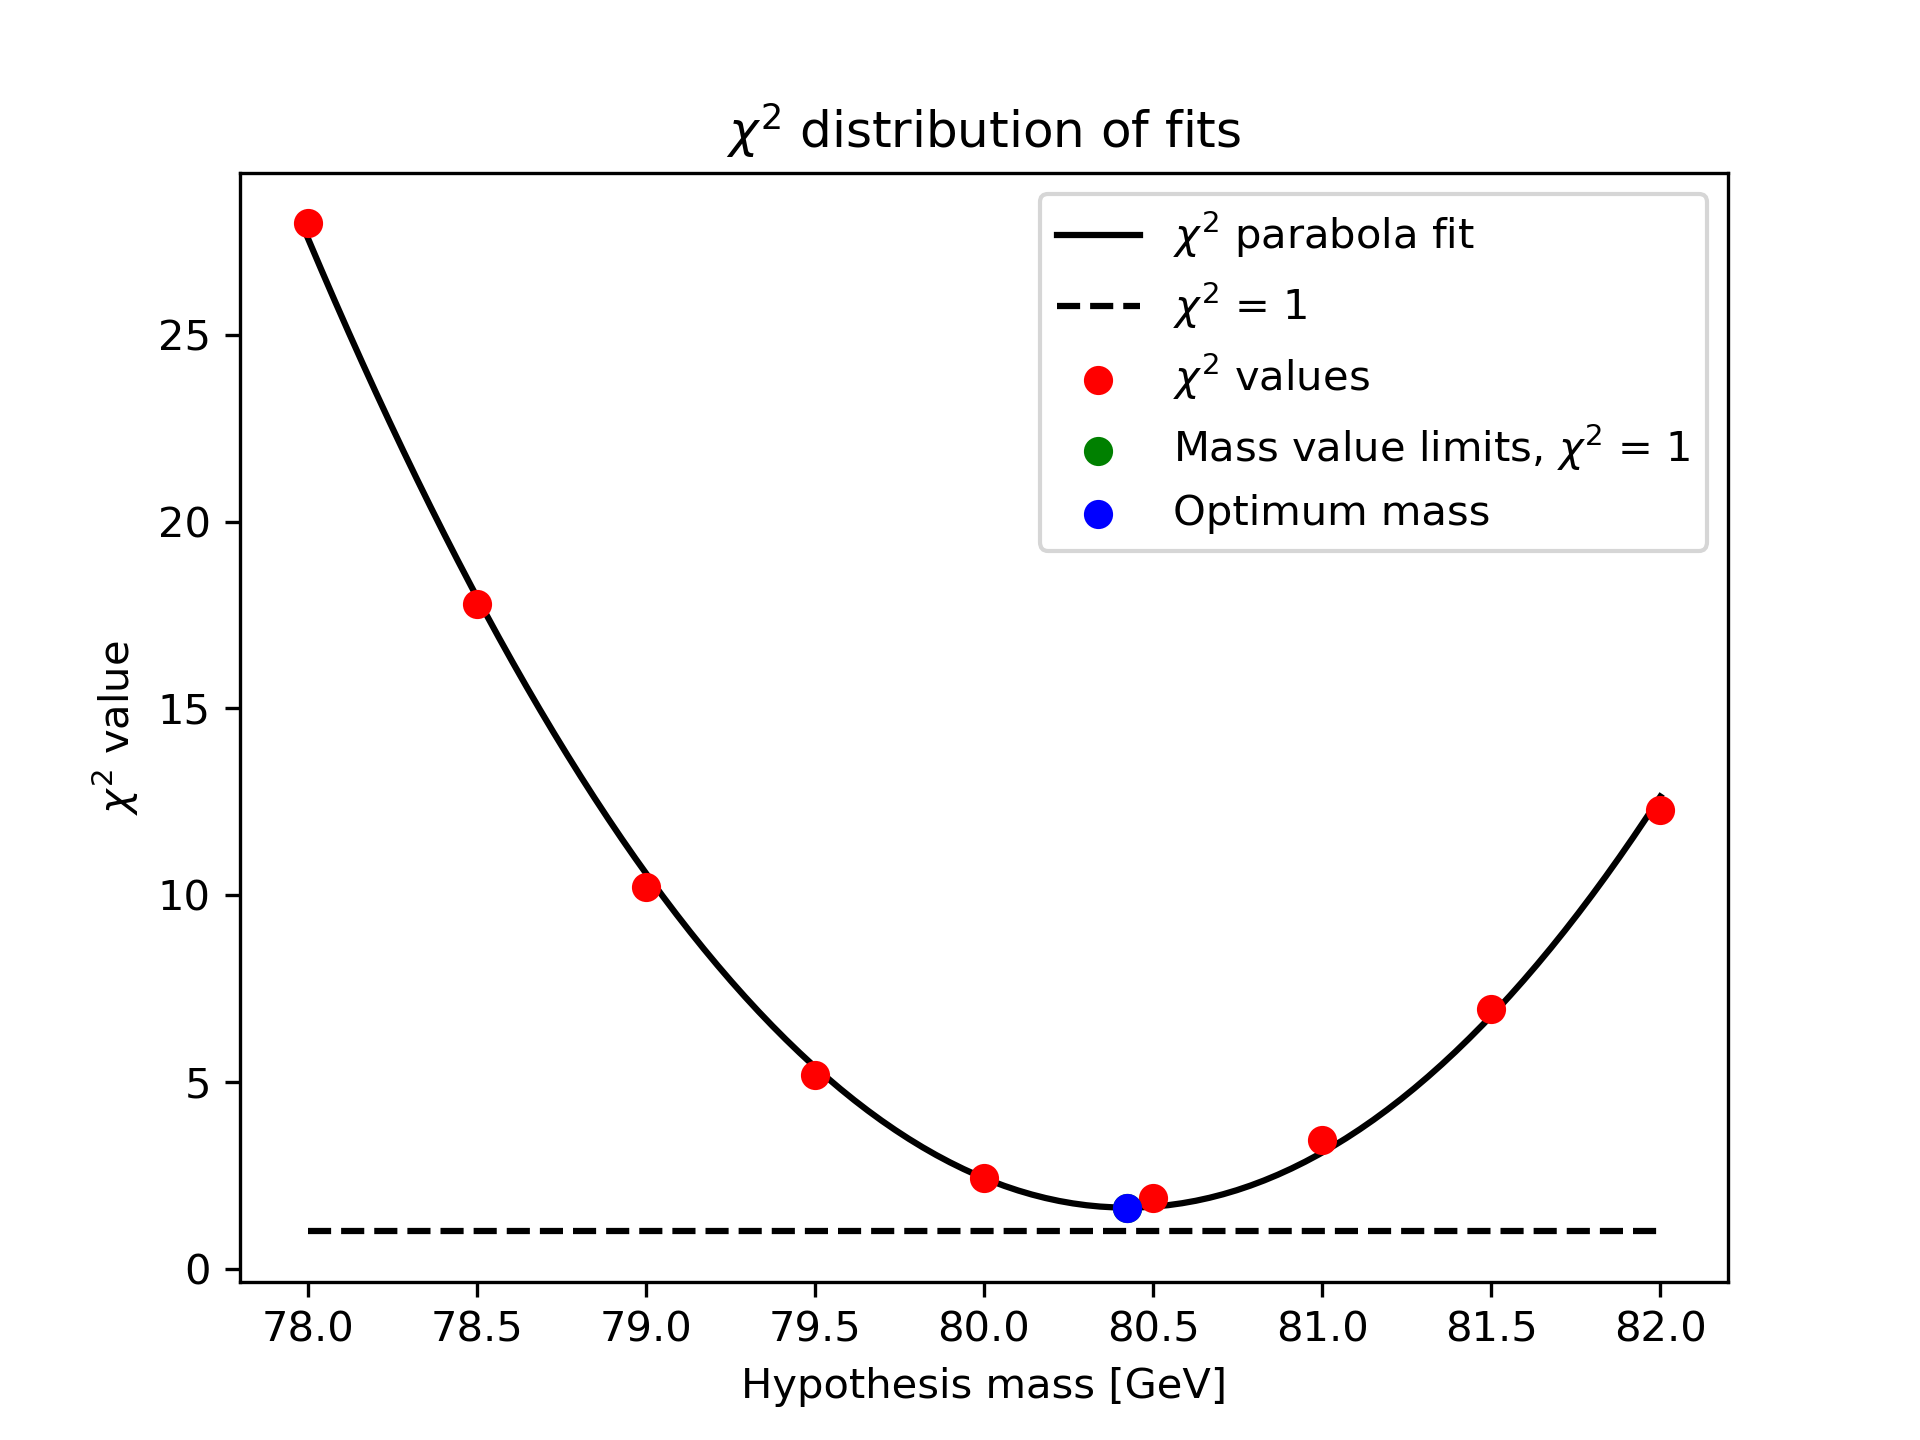
\includegraphics[width=\columnwidth]{/home/physics/phuxdp/Desktop/PX402 Physics Project/WBosonProject/T2W5/plots/chi_square_fits_muPT_80.379_2.07_between_78_and_82_summary.png}
		\caption{\small $\chi^2$ of hypothesis masses. }
		\label{fig: fig_chi_square}
	\end{figure}

    \begin{figure}[tb]
		\centering
		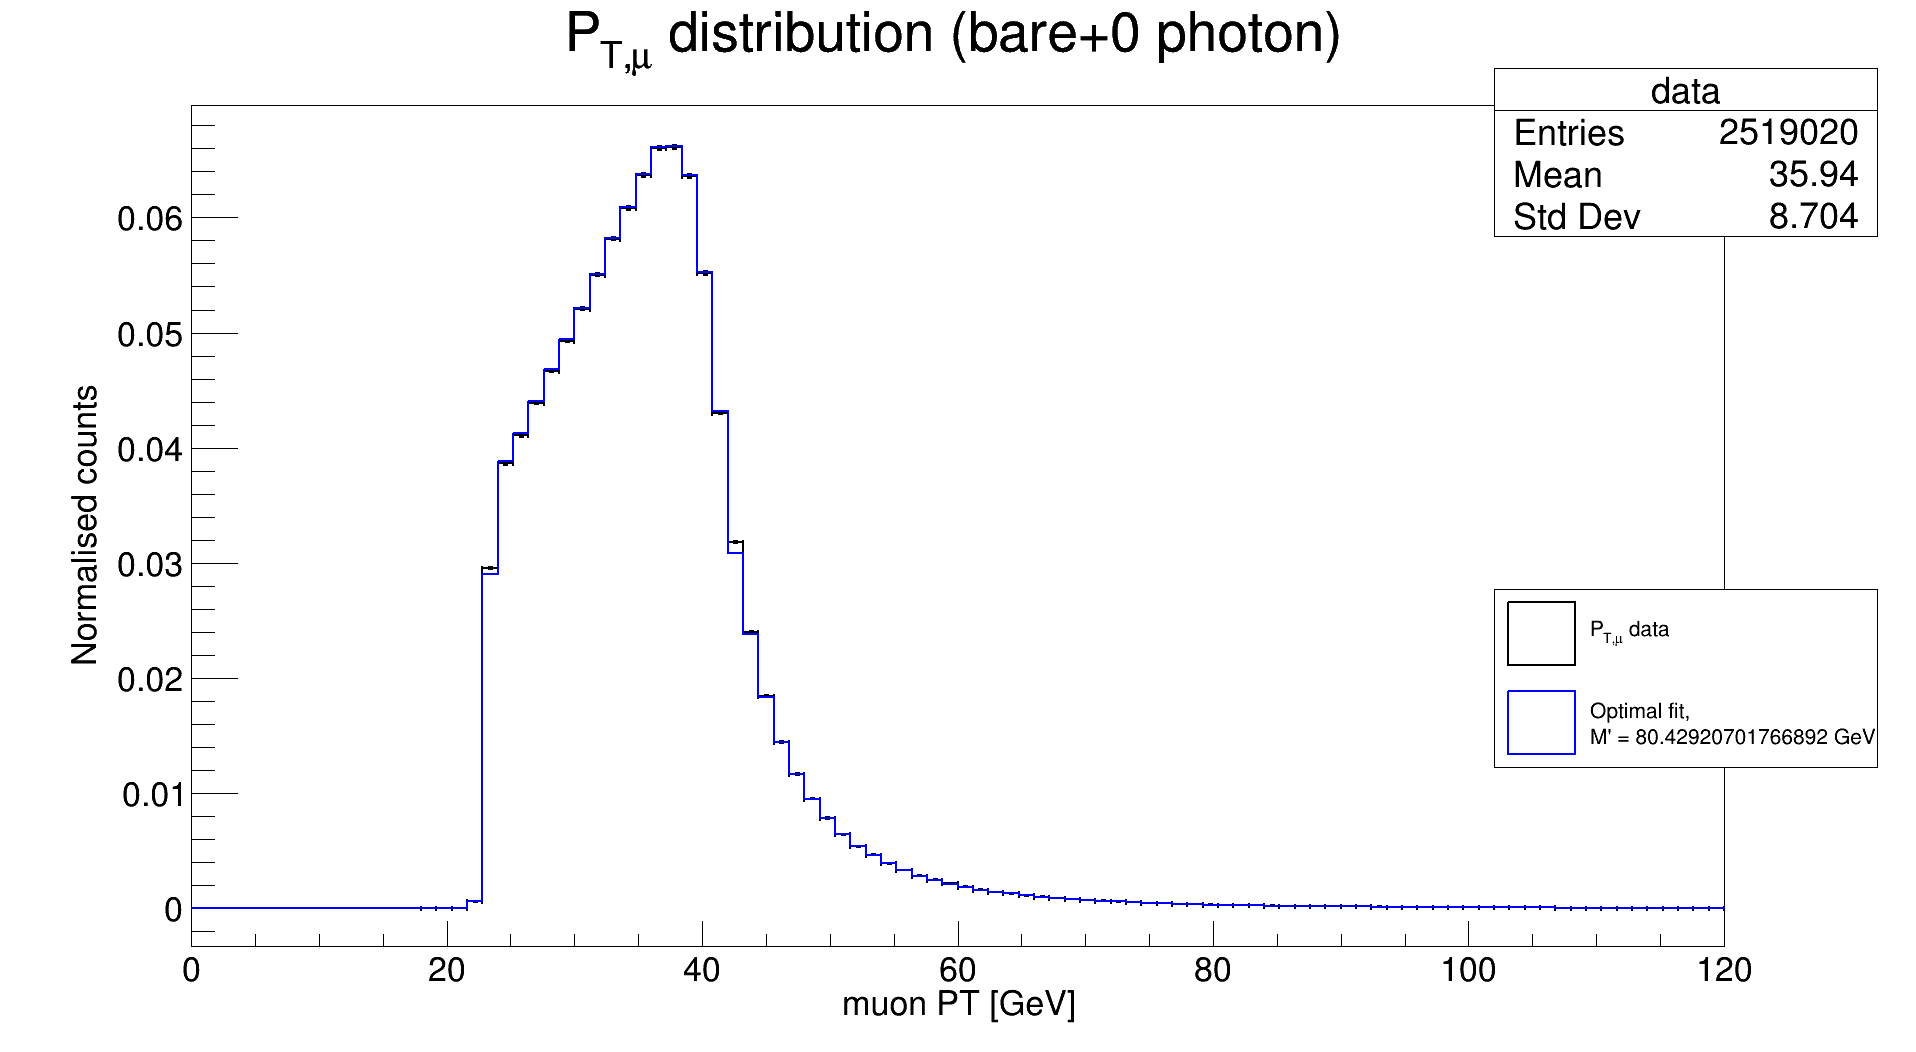
\includegraphics[width=\columnwidth]{/home/physics/phuxdp/Desktop/PX402 Physics Project/WBosonProject/T2W5/plots/optimum_muPT_80.379_2.07_between_78_and_82_summary.png}
		\caption{\small Data and optimum fit with $\chi^2 = 0.039836127173508484$. Used the hypothesis mass of 81.11190200172251$\pm$0.0 $[GeV/c^{2}]$. }
		\label{fig: fig_optim_parms}
	\end{figure}
    
\end{document}